%!TEX root = ../MasterThesis.tex

\section{System Design Proposal}
\label{sec:design_proposal}

As the previous section showed, existing approaches are of limited use for the design of a collaborative system to support the \gls{E-commerce} fraud investigation scenario described in Section~\ref{sec:scope_thesis}. The leading approach for such a system will have to combine the best characteristics from the Web Service and the Semantic Web designs. \\

As for the Web Service approach, the most valuable aspects of it are: \@

\begin{itemize}
	\item access to the \gls{HTTP} endpoints can be limited to a certain set of communication partners
	\item these partners have to authenticate with each Web Service first
	\item based on the identification of the partners only certain parts of information can be returned, and execution of operations can be restricted
\end{itemize}

Looking at the Semantic Web approach, it's most interesting functionalities are: \@

\begin{itemize}
	\item providing information in a semantically self-contained way
	\item the ability to merge information from different \gls{RDF} data stores locally
	\item the graph-based data model underlying the \gls{RDF} data stores
	\item the usage of \gls{SPARQL} to query and analyze the locally combined data sets
\end{itemize}

In the following section the thesis will come up with an approach, that uses the fundamental technologies from the Semantic Web for information sharing and integration as well as peer-to-peer communication technologies for securing and restricting access to the \gls{RDF} data sets from the relevant participants of the \gls{E-commerce} fraud investigation scenario. It will start with a discussion of the semantics of the underlying \gls{RDF} data sets and how these can be combined across various organizations. After that it shows how these information can be provided to the relevant parties in the \gls{E-commerce} fraud investigation scenario. For this purpose it will have a detailed look into the partially centralized \gls{P2P} communication architecture and show how that can be used for the proposed solution.

\subsection{Vocabulary alignment}
\label{subsec:vocab_align}

Although the \gls{RDF} format has build-in support for merging information from different data sources, this functionality is only working as expected if the ``triples'' in the dispersed data stores are using the same \gls{URI}s to refer to the same subjects or objects. In that case merging the ``triples'' from different \gls{RDF} data files will result in a local graph holding the combined information as shown in Figure~\ref{fig:images_combine_rdf_graph}. \\

\begin{figure}[!ht]
	\centering
		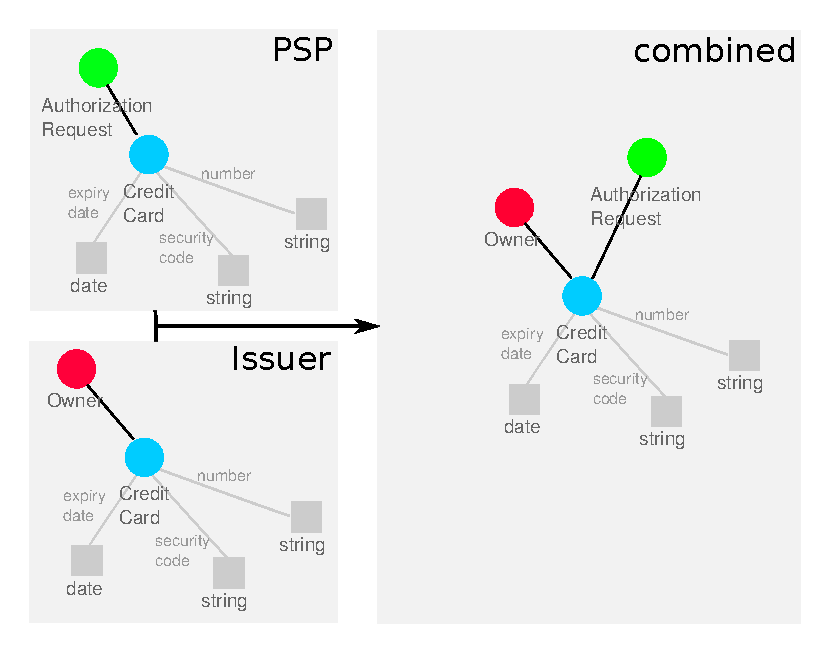
\includegraphics[width=0.9\columnwidth]{images/combine_rdf_graph.pdf}
	\caption{Combining two \gls{RDF} files containing the same credit card entity}
\label{fig:images_combine_rdf_graph}
\end{figure}

As a major objective of the \gls{E-commerce} fraud investigation system is to bring the various transactional information from online merchants, \gls{PSP}s and issuers together, combine them and analyze the resulting graph from different view points, the information exchanged between the relevant participants either have to follow a common schema or have to be mapped against each other.

\subsubsection{Defining a common schema}
\label{subsub:rdf_schema_design}

A common approach would be to define a completely new schema for the proposed system and share that with every possible stakeholder. This schema will define all the entities and relations known to the collaborative system and would be expressed in \gls{RDFS} format. A major drawback of this approach is, that new partners of the system will first have to implement the conversion of their internal data structures to an \gls{RDF} data set, that is compatible with the specific schema definition, before being able to participate in it. \\

Therefore a better approach is to take a look into commonly used \gls{RDF} schemata and vocabularies, and try to figure out whether they can be used for describing the information, that need to be exchanged between participants of the \gls{E-commerce} fraud investigation system. When consulting the Semantic Web community for commonly agreed upon and highly used \gls{RDF} schema specifications, one will come up with this list (see Table~\ref{tab:used_vocab_rdf}):\@

\begin{table}[H]
\centering
\begin{tabular}{p{3cm}llp{4.5cm}}
\hline
\textbf{Name} & \textbf{Prefix} & \textbf{Describes} & \textbf{Namespace URI} \\
\hline
Dublin Core & dc: & Meta data & \url{http://purl.org/dc/terms/} \\
\hline
FOAF & foaf: & People & \url{http://xmlns.com/foaf/0.1/} \\
\hline
Geo & pos: & Positions & \url{http://www.w3.org/2003/01/geo/wgs84\_pos\#} \\
\hline
Geo Names & gn: & Locations & \url{http://www.geonames.org/ontology\#} \\
\hline
Good Relations & gr: & Products & \url{http://purl.org/goodrelations/v1\#} \\
\hline
RDF & rdf: & Core framework & \url{http://www.w3.org/1999/02/22-rdf-syntax-ns\#} \\
\hline
RDFS & rdfs: & RDF vocabularies & \url{http://www.w3.org/2000/01/rdf-schema\#} \\
\hline
Schema.org & schema: & Schema.org vocabularies & \url{http://schema.org/} \\
\hline
SKOS & skos: & Controlled vocabularies & \url{http://www.w3.org/2004/02/skos/core\#} \\
\hline
vCard & vcard: & Business Cards & \url{http://www.w3.org/2006/vcard/ns\#} \\
\hline
Web Ontology Language & owl: & Ontologies & \url{http://www.w3.org/2002/07/owl\#} \\
\hline
XML Schema Datatypes & xsd: & Data types & \url{http://www.w3.org/2001/XMLSchema\#} \\
\hline
\end{tabular}
\caption[Commonly used \gls{RDF} vocabularies on the Web]{Commonly used \gls{RDF} vocabularies on the Web \citep[pg. 41]{wood2014linked}}
\label{tab:used_vocab_rdf}
\end{table}

Based on these schema specifications describing a fictive consumer named ``Max Mustermann'' incl.\ his home address can be done by combining data utilizing the \gls{FOAF} and \gls{vCard} namespaces in a \gls{RDF} data set, such as described in Listing~\ref{lst:sample_customer_mustermann} and visualized as graph in Figure~\ref{fig:images_sample_customer}. \@

\begin{listing}[H]
  \inputminted[linenos,
               numbersep=5pt,
               breaklines=true,
               frame=lines]{TURTLE}
               {./samples/sample_customer_mustermann.ttl}
  \caption{Personal related information about a fictive consumer in \gls{RDF}}
\label{lst:sample_customer_mustermann}
\end{listing}

\begin{figure}[H]
	\centering
		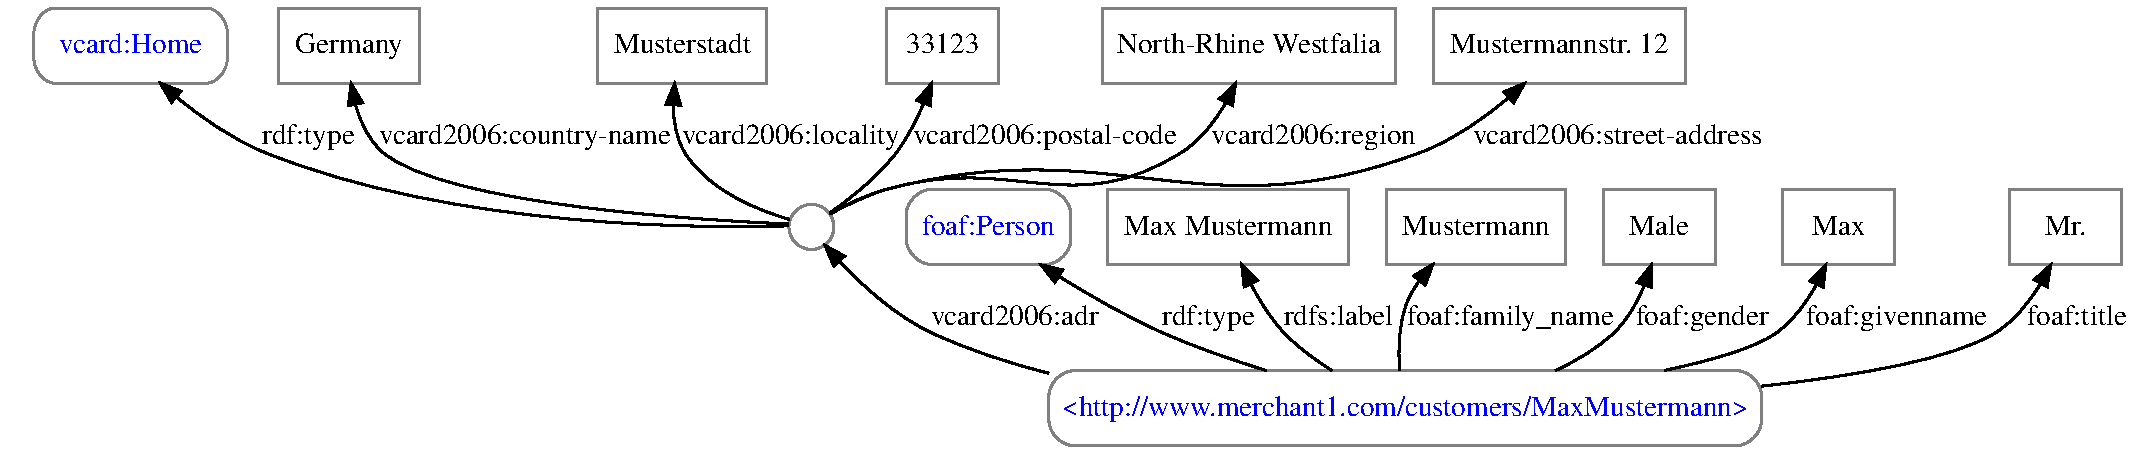
\includegraphics[width=\columnwidth]{images/sample_customer_mustermann.pdf}
	\caption{Graph representation of consumer information from Listing~\ref{lst:sample_customer_mustermann}}
\label{fig:images_sample_customer}
\end{figure}

Looking back to the initial data model from Section~\ref{sec:system_concept} one can map the information, that are currently available in the \gls{E-commerce} scenario, to the existing \gls{RDF} vocabularies such as follows (see Table~\ref{tab:map_tx_rdf_vocab}):\@

\begin{table}[H]
\centering
\begin{tabular}{p{5cm}l}
\hline
\textbf{Information} & \textbf{RDF vocabulary} \\
\hline
Consumer & FOAF \\
\hline
Credit Card Owner & FOAF \\
\hline
Billing Address & vCard \\
\hline
Shipping Address & vCard \\
\hline
Location Information & Geo Names \\
\hline
Merchant & GoodRelations \\
\hline
Items & GoodRelations \\
\hline
Item Categories & GoodRelations \\
\hline
Brands & GoodRelations \\
\hline
Payment Types & GoodRelations \\
\hline
\end{tabular}
\caption{Possible usage of \gls{RDF} vocabularies for \gls{E-commerce} transaction information}
\label{tab:map_tx_rdf_vocab}
\end{table}

As this table shows there are some parts of the \gls{E-commerce} data model that can be expressed with existing \gls{RDF} vocabularies extensively --- such as personal related information via \gls{FOAF} and \gls{vCard}, whereas other parts can not be stated in-depth (e.g. credit card information), or are not specified at all (e.g.\ tracking of the delivery). Additionally some of the vocabularies are no longer actively maintained, such as GoodRelations. Due to these circumstances one usually have to build an own ontology that fills in the missing pieces and refers to the existing concepts whenever appropriate. Trying to model the information of a credit card as displayed in Figure~\ref{fig:images_data_model} will result in the \gls{RDFS} specification shown in Listing~\ref{lst:credit_card_vocab}. This definition of a credit card resource explicitly reuses specifications from the \gls{FOAF} and GoodRelations ontologies by specifying that: \@

\begin{itemize}
	\item the owner of a credit card has to be of type ``Person'' from the \gls{FOAF} ontology
	\item the type of a credit card has to be an instance of the type ``PaymentMethodCreditCard'' from the GoodRelations ontology
\end{itemize}

\begin{listing}[H]
  \inputminted[linenos,
               numbersep=5pt,
               breaklines=true,
               frame=lines]{TURTLE}
               {./samples/vocab_credit_card.ttl}
  \caption{A specification for a credit card in \gls{RDFS}}
\label{lst:credit_card_vocab}
\end{listing}

As most of the parts of the \gls{E-commerce} data model shown in Figure~\ref{fig:images_data_model} can not be expressed with the existing \gls{RDF} vocabularies, filling in the gaps would mean to come up with a large set of custom entities and relationships. As stated above, this will limit the general usage of the collaborative system. When looking back at the list of existing ontologies and vocabularies, that are actively used on the Web today, one will find the Schema.org vocabulary definition \citep{Schema.org}. This vocabulary was initially designed by the leading search engines (aka Google, Microsoft and Yahoo!) to allow authors of Web sites to markup their \gls{HTML} documents in a way, that they are better understood by those search engines. The Schema.org vocabulary is actively maintained by its community, includes new concepts with each release and also offers an extension mechanism to implement additional vocabularies, that are not part of the core specification \citep{SchemaExtensions}. In one of the past releases of the Schema.org core specification the maintainers also included all of the existing concepts of the GoodRelation ontology into the Schema.org vocabulary \citep{SchemaGoodRelation}. \\

As the merchants will have to provide semantic meta data for their products to improve their listings on search engine results (also known as \gls{SEO}) in the vocabulary of Schema.org already, one can re-use parts of these information for the \gls{E-commerce} fraud investigation scenario. Additionally, the wide-ranging scope of aspects that Schema.org declares, make it a good fit for the collaborative system in the \gls{E-commerce} fraud investigation scenario as one can assume that each participant is aware of this meta data initiative and the relevant communication partners will have a common understanding of the terms used within the system. When trying to map the initial data model from Section~\ref{sec:system_concept} to the Schema.org core specification one will basically come up with a data schema as displayed in Figure~\ref{fig:images_schema_org}. \@

\begin{figure}[!ht]
	\centering
		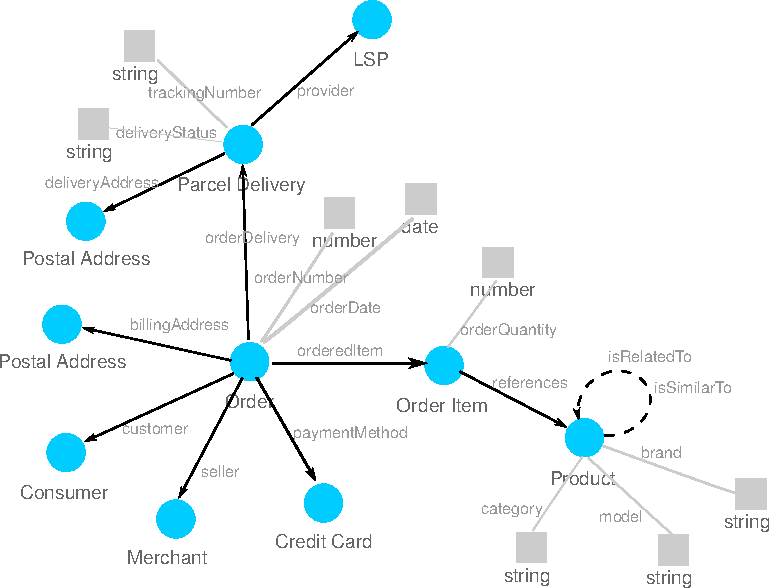
\includegraphics[width=0.8\columnwidth]{images/schema_org_mapping.pdf}
	\caption{Schema.org based mapping of an \gls{E-commerce} transaction}
\label{fig:images_schema_org}
\end{figure}

\subsubsection{Mapping of the information}
\label{subsub:rdf_mapping_information}

Although it is possible to model each \gls{E-commerce} transaction with the Schema.org specification as shown in Figure~\ref{fig:images_schema_org}, the collaborative system still has to take care of the mapping of the transactional information coming from various sources to be able to analyze and cluster them. As shown in the Section~\ref{subsec:vocab_align} the build-in merging capabilities of the \gls{RDF} specification rely on the \gls{URI}s used for the entities in the various \gls{RDF} data sets. These \gls{URI}s are used to uniquely identify the resources in a \gls{RDF} data set. \\

The \gls{W3C} standards for the Semantic Web also include support for the mapping issues, that will also come up when trying to combine semantic information available on the Web. Additionally, the Schema.org specification defines properties that can be used for that purpose. The following concepts are available in the \gls{RDFS}, \gls{OWL} and Schema.org specifications: \@

\begin{itemize}
	\item \textbf{rdfs:label}: a label of a resource in the \gls{RDF} data set can contain a human-friendly name of the resource. These labels are literals of type string and can come with a language specifier in case the resource supports expressions for different languages (see Listing~\ref{lst:rdfs_label_language} for an example).
	\item \textbf{rdfs:seeAlso}: a relation of type seeAlso contains an \gls{URI} to an external resource, that contains additional information for the subject (see Listing~\ref{lst:rdfs_seeAlso_location} for an example).
	\item \textbf{rdfs:isDefinedBy}: the isDefinedBy property is a specialization of the seeAlso relation, in that it specifies a link to the original definition of a resource
	\item \textbf{owl:sameAs, schema:sameAs}: the sameAs relation as specified in the \gls{OWL} and Schema.org vocabularies are providing an unique \gls{URI} that unambiquiously define the subject (see Listing~\ref{lst:schema_sameAs_location} for an example)
\end{itemize}

\begin{listing}[H]
  \inputminted[linenos,
               numbersep=5pt,
               breaklines=true,
               frame=lines]{TURTLE}
               {./samples/sample_product_with_labels.ttl}
  \caption[Specifying a product with labels in three different languages in \gls{RDF}]{Specifying a product with labels in three different languages in \gls{RDF}\protect\footnotemark}
\label{lst:rdfs_label_language}
\end{listing}

\footnotetext{Please note that the name of the product has been stated without a language specifier, which means global usage of it.}

\begin{listing}[H]
  \inputminted[linenos,
               numbersep=5pt,
               breaklines=true,
               frame=lines]{TURTLE}
               {./samples/sample_customer_location.ttl}
  \caption[Specifying a link to a Geo Names resource for looking up additional location information in \gls{RDF}]{Specifying a link to a Geo Names resource for looking up additional location information in \gls{RDF}\protect\footnotemark}
\label{lst:rdfs_seeAlso_location}
\end{listing}

\footnotetext{Please note that the application has to resolve the \gls{URI} and embedd the resulting \gls{RDF} data set at this position in the graph.}

\begin{listing}[H]
  \inputminted[linenos,
               numbersep=5pt,
               breaklines=true,
               frame=lines]{TURTLE}
               {./samples/sample_customer_location2.ttl}
  \caption{Specifying a link to a DBpedia resource to uniquely identify an entity in \gls{RDF}}
\label{lst:schema_sameAs_location}
\end{listing}

When looking at the \gls{E-commerce} transaction schema as defined in Section~\ref{sec:system_concept} the following information must be uniquely identified and mapped in the \gls{RDF} data sets from the participants of the collaborative system: \@

\begin{itemize}
	\item \textbf{personal related information} such as the consumer, recipient and credit card owner
	\item \textbf{location based information} such as the billing and shipping address as well as the location a credit card owner is registered for
	\item \textbf{product related information} such as the categories, subcategories, brand, model and item description
	\item \textbf{merchant related information} such as the branch
\end{itemize}

To support the unique identification of entities in the \gls{RDF} data set of an \gls{E-commerce} transaction one can refer to publicly available \gls{RDF} data sets on the Internet, such as GeoNames or DBpedia. These will provide an unique \gls{URI} for locations and named places. A product-related \gls{RDF} data set was available in form of the ProductDB initiative until recently \citep{bouzidi2014product}. Due to this the mapping of products can no longer be done by referencing unique \gls{URI}s, but will have to be based on the global trade item number (aka \gls{GTIN}). Additional aspects of an item, such as brand, categories and subcategories, can be found on DBpedia. A problem, that will come up, is the unique addressing of personal related information, such as identifying the consumer. The collaborative system can not rely on mapping the personal related information based on properties such as familyName and givenName alone (see Listing~\ref{lst:sample_customer_mustermann}). There could be typos in the information coming from various \gls{RDF} data sets, and different individuals can still have the same name information. One possible approach to bring these information together would be the mapping based on the e-mail address of the individual. An e-mail address like an \gls{URI} is a globally unique addressing scheme, and one can assume that two entities, who are using to the same e-mail address, are referring to the same entity. Still this is a weak hint as an individual can have more than one e-mail address, and could use different e-mail addresses for the online shopping trips at different merchants. Therefore a more sophisticated mapping algorithm for personal related information is needed in the collaborative system. This algorithm may take into account the combination of familyName, givenName, dateOfBirth as well as location-based information to uniquely identify an individual.

% subsec vocab_align

\subsection{Communication protocols}
\label{subsec:comm_protocol}

 The data is likely encoded in Microdata, \gls{RDFa} or \gls{JSON-LD}. \\

For the communication the \gls{WebRTC} is a good approach as it integrates well with existing enterprise IT infrastructures.
\\

\ldots

% subsec comm_protocol

\subsection{Designing a partially centralized \gls{P2P} system}
\label{subsec:p2p_partially_centralized_system}

For the \gls{E-commerce} fraud scenario, that has been selected for this thesis in Section~\ref{sec:thesis_scope}, one can say that the issuer of a credit card is the party who initiates the collaborative fraud investigation. They are recognizing the active use (and likely misuse) of a credit card in the online and the offline world first, and are also getting a notification about any suspicious transactions made with it from their fraud prevention systems. Due to this fact, one can come up with a partially centralized \gls{P2P} architecture for the \gls{E-commerce} fraud investigation system, in that the issuer of a card in at the center and acts as a trusted party in this system. This issuer will initiate a collaborative session with the other required stakeholders based on the usage history of the credit card in question. During this \gls{P2P} communication session the merchants, \gls{PSP}s and \gls{LSP}s will share the required information with the issuer. In this process the data from the other stakeholders will be replicated to the issuer, who will build up a networked graph based on the Schema.org specification. So the main work will be on the issuer's side, who is the major driving party in the system, as depicted in Figure~\ref{fig:images_p2p_centralized}.\@

\begin{figure}[H]
	\centering
		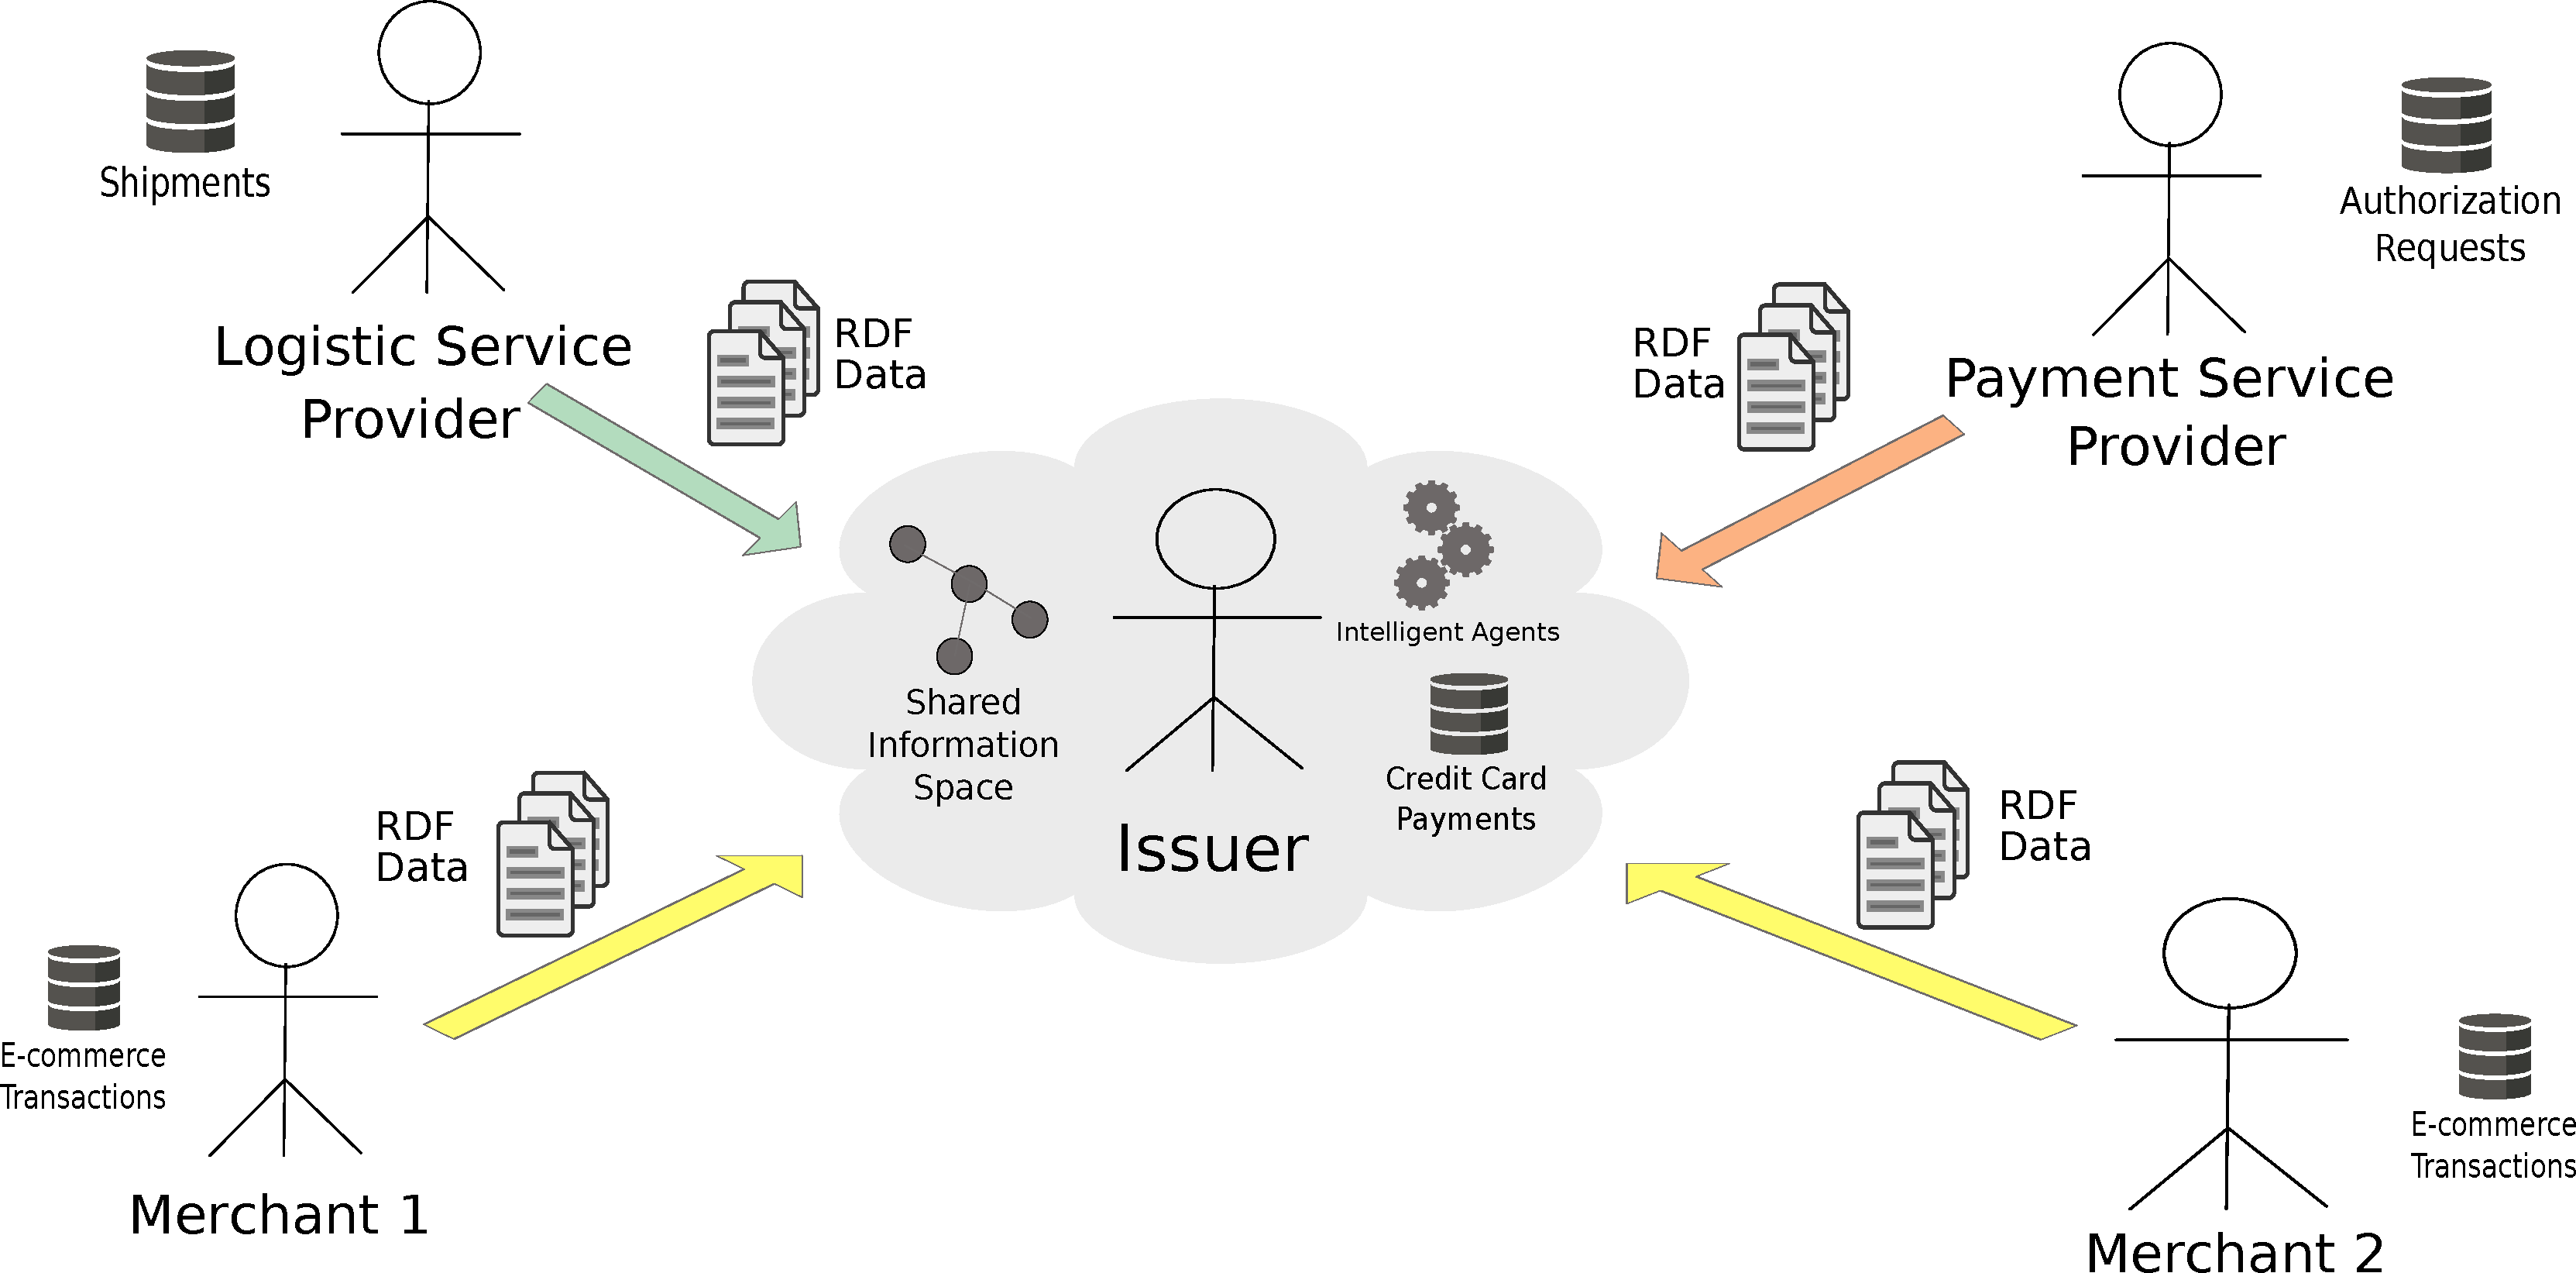
\includegraphics[width=0.9\columnwidth]{images/system_P2P_centralized.pdf}
	\caption{Collaborative system using a partially centralized \gls{P2P} architecture}
\label{fig:images_p2p_centralized}
\end{figure}

Using the \gls{WebRTC} communication protocol for initiating the \gls{P2P} session will allow the issuers to setup a communication between the relevant stakeholders directly from within an application running in their Web browsers. The application can visualize the connectivity status of the participants, the progress of their data sharing efforts as well as offer direct face-to-face communication possibilities in case of misunderstandings or further requests. A wireframe of the Web application screen is depicted in Figure~\ref{fig:images_p2p_initial_screen}. \@

\begin{figure}[H]
	\centering
		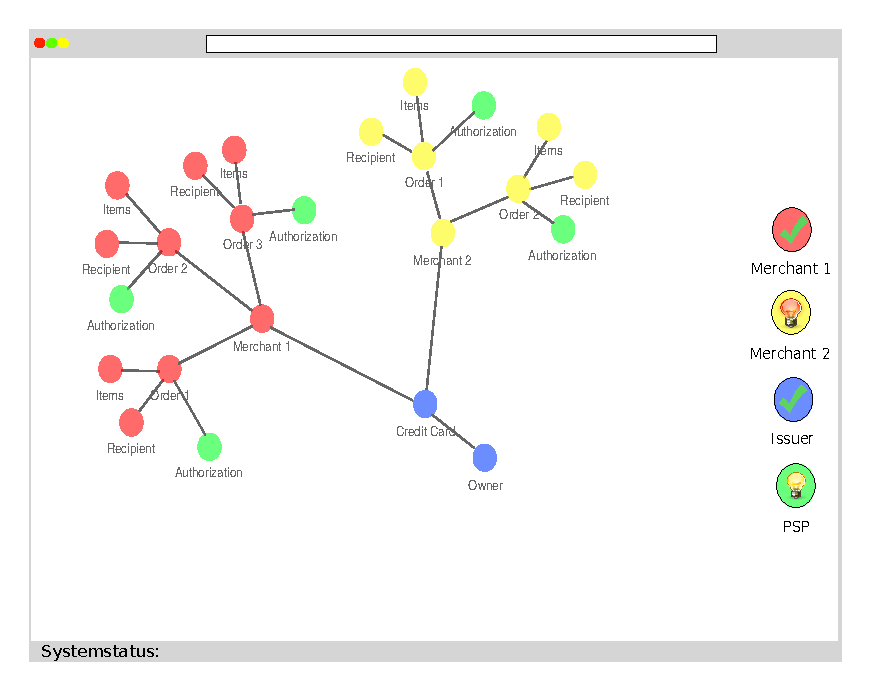
\includegraphics[width=0.9\columnwidth]{images/p2p_initial_screen.pdf}
	\caption{Screen prototype of collaborative system showing participants and shared information}
\label{fig:images_p2p_initial_screen}
\end{figure}

One of the major issues with the above mentioned system architecture is, that the merchants, \gls{PSP}s and \gls{LSP}s have to hand over all of their relevant information to the issuer of a credit card for the analysis. \\

\ldots

% subsec p2p_partially_centralized_system

% section design_proposal (end)
